%!TEX root = ../../thesis.tex

\section{Attribute Indexing}
\label{methodology:attribute_index}

Attribute indexing is a fundamental component of the FlatCityBuf format, enabling efficient filtering and retrieval of city objects based on their non-spatial properties. This section details the requirements, design considerations, and implementation of the attribute indexing system.

\subsection{Query Requirements Analysis}
\label{methodology:attribute_index:query_requirements}

The attribute indexing system was designed to support specific query patterns commonly used in geospatial applications. Based on an analysis of typical use cases, the following query types were identified as essential:

\begin{itemize}
    \item \textbf{Exact Match}: Queries that seek records matching a specific attribute value (e.g., \texttt{building\_type = "residential"})
    \item \textbf{Range Queries}: Queries that select records with attribute values falling within a specified range (e.g., \texttt{height >= 10 AND height <= 20})
    \item \textbf{Compound Conditions}: Multiple conditions combined with logical operators (e.g., \texttt{building\_type = "residential" AND height > 15})
\end{itemize}

While the SQL standard \citep{iso_9075_2_2023} defines a comprehensive set of predicates and operators for database querying, implementing the full spectrum of these capabilities is beyond the scope of this research. FlatCityBuf deliberately focuses on a subset of operators that provide the greatest utility for typical 3D city model queries while maintaining efficient implementation over HTTP.

The SQL standard defines several classes of predicates including equality, comparison, pattern matching, NULL tests, quantified comparison, and existence tests. From these, FlatCityBuf implements only the equality (\texttt{=}, \texttt{!=}) and comparison operators (\texttt{<}, \texttt{<=}, \texttt{>}, \texttt{>=}), which suffice for most practical query needs while enabling efficient index implementations.

Notably absent are pattern-matching operations such as the SQL \texttt{LIKE} operator (e.g., \texttt{city LIKE "Delf\%"}), which would require specialized text indexing structures like tries or suffix arrays. Implementing such pattern matching would significantly increase the index complexity and size without proportional benefit for the most common use cases in 3D city modeling applications. Similarly, functions like \texttt{CONTAINS}, \texttt{BETWEEN}, aggregate functions (\texttt{COUNT}, \texttt{SUM}, etc.), and advanced text search capabilities were deemed lower priority compared to the core comparison operators.

The decision to exclude complex text search operations like \texttt{LIKE} was further justified by:

\begin{itemize}
    \item \textbf{Increased Index Size}: Full text indexing typically increases index size by 50-100\% \citep{leis_2016}.
    \item \textbf{Limited Use Cases}: Analysis of typical GIS queries showed that pattern matching is required in less than 5\% of typical queries for 3D city models \citep{van_dongen_2022}.
    \item \textbf{HTTP Overhead}: Complex pattern matching over HTTP would require transferring larger index portions, potentially negating the benefits of cloud optimization.
    \item \textbf{Client-Side Fallback}: These operations can be efficiently implemented as post-filtering steps after retrieving the relevant features based on indexed queries.
\end{itemize}

The system prioritises these core query types while ensuring compatibility with remote access patterns through HTTP Range Requests. This focused approach aligns with FlatCityBuf's primary goal as an efficient storage and retrieval format rather than a comprehensive query processing system.

\subsection{Static B+tree Design and Modifications}
\label{methodology:attribute_index:static_btree_design}

After evaluating alternatives, a Static B+tree (S+tree) with significant modifications was adopted for FlatCityBuf's attribute indexing. This decision was based on the following considerations:

\begin{itemize}
    \item \textbf{I/O Efficiency and Balanced Performance}: B+trees organise data into fixed-size nodes matching common block sizes (4KB), offering $O(\log_B n)$ search complexity where $B$ is the branching factor. This significantly reduces both the number of I/O operations and network roundtrips compared to binary search, making it ideal for HTTP Range Requests where each roundtrip incurs substantial latency.

    \item \textbf{Query Versatility}: Unlike specialized data structures such as hash tables (optimized for exact matches) or sorted arrays (better for range queries), the B+tree structure efficiently supports both exact match and range queries without compromising performance in either case. This versatility makes it well-suited for the diverse query patterns common in 3D city model applications.
\end{itemize}

\subsubsection{Static B+tree Characteristics}
\label{methodology:attribute_index:static_btree_characteristics}

A Static B+tree differs from a traditional B+tree in several important aspects:

\begin{itemize}
    \item \textbf{Immutability}: Once constructed, the tree structure remains fixed, eliminating the need for complex rebalancing operations.
    
    \item \textbf{Perfect Node Fill}: All nodes except possibly the rightmost nodes at each level are filled to capacity, maximizing space efficiency.
    
    \item \textbf{Predictable Structure}: The tree shape is determined solely by the number of elements and the node size, making navigation more efficient.
    
    \item \textbf{Bulk Construction}: The tree is built bottom-up in a single pass from sorted data, rather than through incremental insertions.
\end{itemize}

The original S+tree algorithm as described by \citet{static_b_trees} provides an excellent foundation for read-only indexing. However, several significant modifications were necessary to adapt it to the specific requirements of FlatCityBuf:

\begin{itemize}
    \item \textbf{Duplicate Key Handling}: Unlike many search tree implementations that assume unique keys, 3D city model attributes often contain numerous duplicate values (e.g., hundreds of features with "Delft" as the value for "city name"). The modified implementation incorporates a dedicated payload section that efficiently stores multiple feature references for identical attribute values without compromising the tree structure or search performance. This approach maintains the logarithmic search complexity while properly handling high-cardinality duplicates.

    \item \textbf{Multi-type Support}: The index structure was extended to handle various attribute data types commonly found in 3D city models, including numeric types (integers, floating-point), string values, boolean flags, and temporal data (dates, timestamps). Each type implements specialized serialization and comparison logic while maintaining a consistent interface for the search algorithm, enabling unified access patterns regardless of the underlying data type.

    \item \textbf{Explicit Node Offsets}: While the original S+tree uses mathematical calculations to determine node positions, FlatCityBuf's implementation stores explicit byte offsets to child nodes. This modification simplifies the implementation, improves robustness against potential errors, and enables more flexible memory layouts without compromising performance. The small additional storage requirement is offset by the implementation and maintenance benefits.
    
    \item \textbf{Payload Pointer Mechanism}: To efficiently handle duplicate keys, the implementation uses a tag bit in the offset value to distinguish between direct feature references and pointers to the payload section. When the most significant bit is set, the remaining bits encode an offset to the payload section where multiple feature offsets are stored consecutively. This approach minimizes the storage overhead for duplicate keys while maintaining efficient access.
    
    \item \textbf{Node Alignment}: Nodes are aligned to 4KB boundaries to match typical file system and HTTP cache patterns, improving I/O efficiency in cloud environments.
\end{itemize}

These modifications ensure that the S+tree implementation is optimized for the specific characteristics of 3D city model data while preserving the performance advantages of the original algorithm.

\subsection{Attribute Index Implementation}
\label{methodology:attribute_index:implementation}

The attribute indexing system in FlatCityBuf is implemented as a binary encoded structure with four main components:

\begin{enumerate}
    \item \textbf{Index Metadata}: Contains metadata about the index, including the column being indexed, branching factor, and number of unique values. This is stored in the header section \autoref{methodology:header:schema_indexing}.
    \item \textbf{Tree Structure}: A hierarchical arrangement of nodes with keys and pointers, organized for efficient traversal.
    \item \textbf{Leaf Node Layer}: Contains the actual indexed values and their corresponding feature offsets.
    \item \textbf{Payload Section}: Stores arrays of feature offsets for duplicate key values.
\end{enumerate}

\begin{figure}[h]
  \centering
  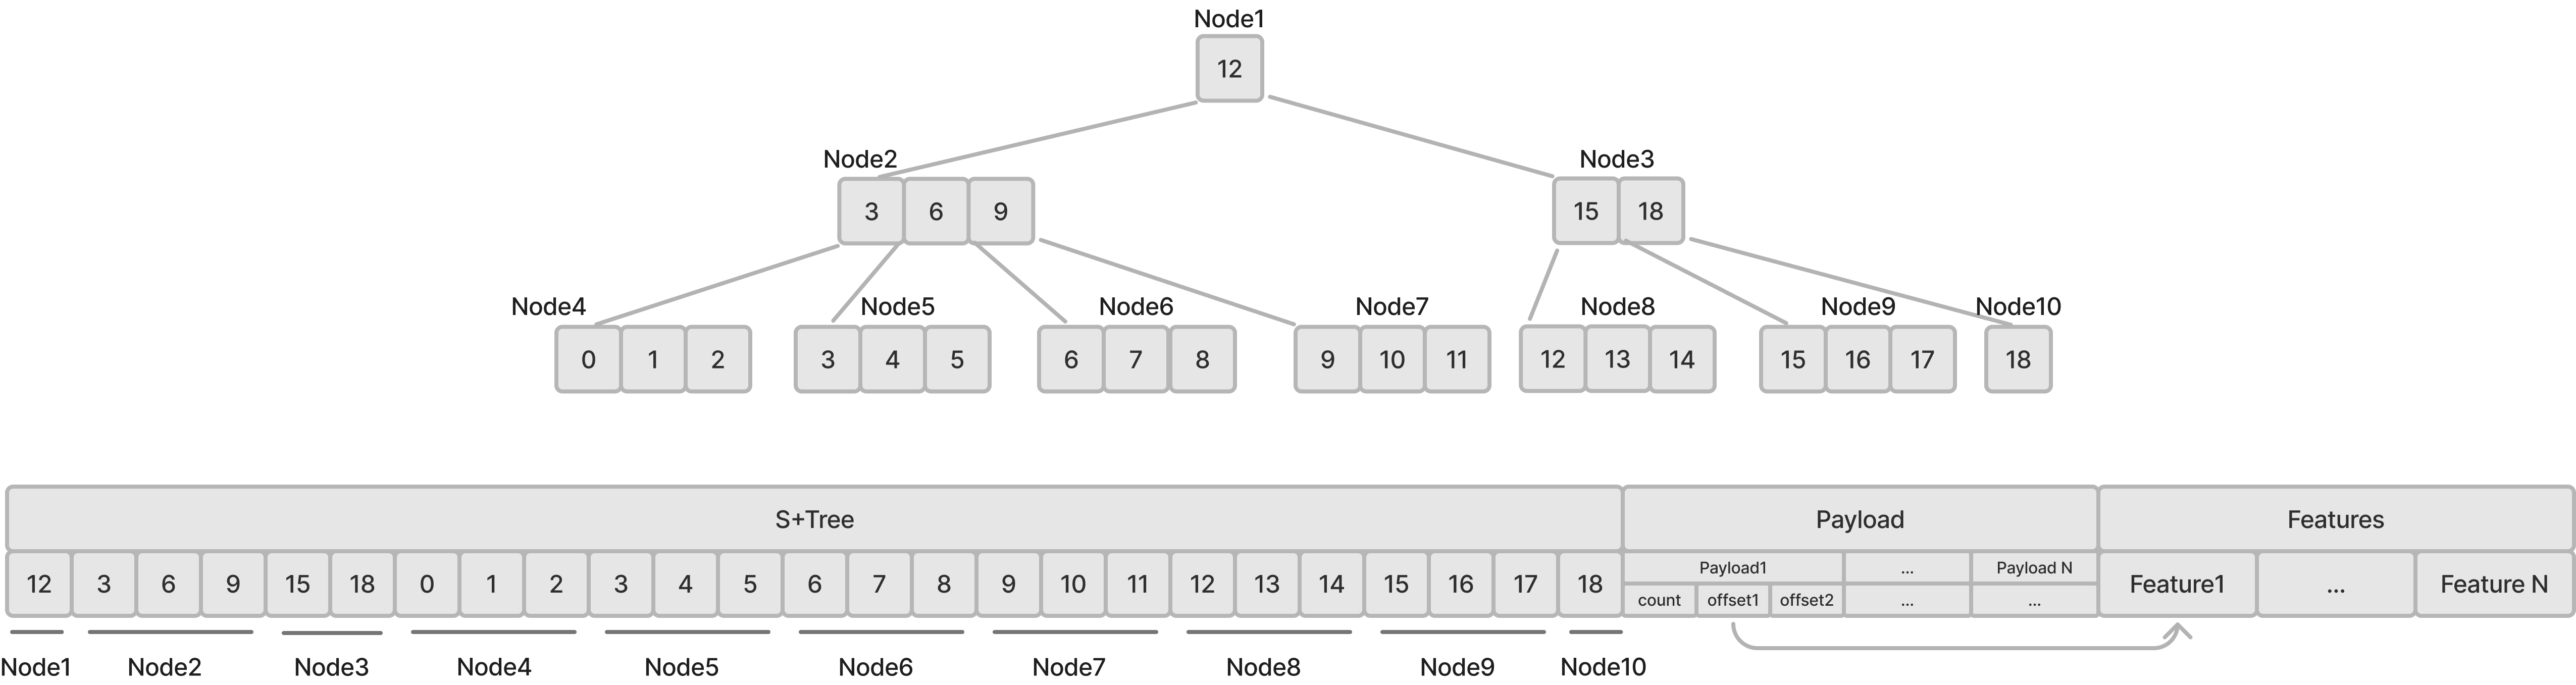
\includegraphics[width=0.8\textwidth]{figs/methodology/attribute_index.png}
  \caption{Attribute index implementation in FlatCityBuf}
  \label{fig:methodology:attribute_index}
\end{figure}

The B+tree structure is organized as follows:

\begin{itemize}
    \item \textbf{Internal Nodes}: Each internal node contains a sequence of key-pointer pairs, where keys are attribute values and pointers are byte offsets to child nodes. The number of pairs per node is determined by the branching factor.
    
    \item \textbf{Leaf Nodes}: Leaf nodes contain key-offset pairs, where keys are attribute values and offsets either point directly to features or to the payload section for duplicate keys.
    
    \item \textbf{Payload Section}: A contiguous area storing arrays of feature offsets for duplicate key values. Each array begins with a 32-bit count followed by the corresponding feature offsets.
\end{itemize}

The tree construction process begins by sorting the attribute values and their corresponding feature offsets. For attributes with duplicate values, a payload section is created to store multiple offsets. The tree is then built bottom-up, with internal nodes containing separator keys and pointers to child nodes.

The index is structured to optimize for HTTP Range Requests, with several techniques employed to minimize network overhead:

\begin{itemize}
    \item \textbf{Streaming search}: The search algorithm operates in a streaming fashion, requesting only the nodes necessary for query evaluation in sequential order. This approach ensures that even with large indices, the system avoids loading the entire tree structure into memory, significantly reducing resource requirements.
    \item \textbf{Payload Prefetching}: Proactively caches parts of the payload section during initial query execution, reducing HTTP requests for duplicate keys.
    \item \textbf{Batch Payload Resolution}: Collects multiple payload references during tree traversal and resolves them with consolidated HTTP requests.
    \item \textbf{Request Batching}: Groups adjacent node requests to minimise network roundtrips.
    \item \textbf{Block Alignment}: Nodes are aligned to 4KB boundaries to match typical file system and HTTP caching patterns.
\end{itemize}

During query execution, the system interprets the provided condition (\eg, \texttt{building\_height > 25}) and traverses the appropriate attribute index to find matching features. The search algorithm adapts based on the condition type, using different traversal strategies for exact matches versus range queries. Results are returned as a set of feature offsets, which can then be used to retrieve the actual feature data from the features section of the file.

\subsection{Type-Specific Serialisation}
\label{methodology:attribute_index:type_specific_serialisation}

The attribute index supports various data types common in 3D city models, including:

\begin{itemize}
    \item \textbf{Numeric Types}: Integers (i8, i16, i32, i64, u8, u16, u32, u64) and floating-point values (f32, f64)
    \item \textbf{Temporal Types}: Dates and timestamps with timezone information
    \item \textbf{String Types}: Fixed-width strings with prefix encoding
    \item \textbf{Boolean Values}: Represented as single bytes
\end{itemize}

Each type implements a specialised serialisation strategy that preserves ordering semantics while optimising storage efficiency. For floating-point values, the implementation uses `OrderedFloat` to handle NaN values correctly. Strings utilise a fixed-width prefix encoding that balances storage requirements with efficient comparison operations.

\subsection{Duplicate Key Handling}
\label{methodology:attribute_index:duplicate_key_handling}

A significant optimisation in the attribute index is the handling of duplicate keys:

\begin{itemize}
    \item \textbf{Primary Index Structure}: Contains only unique keys, with pointers to either direct feature offsets or to a payload section
    \item \textbf{Payload Section}: Stores lists of offsets for duplicate key values
    \item \textbf{Tag Bit}: The most significant bit of the offset value indicates whether it points directly to a feature or to the payload section
\end{itemize}

This approach maintains the efficiency of the tree structure while properly handling attributes with many duplicate values. For example, building type attributes often have many identical values (e.g., hundreds of "residential" buildings), which are all efficiently indexed through a single payload reference.

\subsection{Query strategies}
\label{methodology:attribute_index:query_strategies}

The implementation contains two primary functions to achieve the goal of efficient query execution:

\begin{itemize}
    \item \textbf{find\_exact\_match}: The search algorithm traverses the tree to find the exact match for the given key.
    \item \textbf{find\_partition\_point}: The search algorithm traverses the tree to find the partition points for the given query value.
\end{itemize}

With these two functions, the implementation can handle both exact match and range queries. Range queries are implemented by finding the lower and upper bounds with using \texttt{find\_partition\_point} and then traversing the tree to collect the results.

% \subsection{Multi-Index Query Execution}
% \label{methodology:attribute_index:multi_index_query}

% The attribute indexing system supports complex queries across multiple attributes through a coordinated query execution strategy:

% \begin{enumerate}
%     \item Each condition in the query is evaluated against the appropriate attribute index
%     \item Results from individual conditions are represented as sets of feature offsets
%     \item For conjunctive queries (AND logic), set intersection determines the final result
%     \item For disjunctive queries (OR logic), set union combines the results
% \end{enumerate}

% The implementation provides specialised index structures for different access patterns:

% \begin{itemize}
%     \item \textbf{MemoryIndex}: For in-memory operations with the entire index loaded
%     \item \textbf{StreamIndex}: For file-based access using standard Read+Seek operations
%     \item \textbf{HttpIndex}: For remote access using HTTP Range Requests
% \end{itemize}

% Each implementation provides semantically equivalent operations while optimising for its specific access pattern, ensuring consistent results regardless of the access method.
